\documentclass[3p]{elsarticle} %review=doublespace preprint=single 5p=2 column
%%% Begin My package additions %%%%%%%%%%%%%%%%%%%
\usepackage[hyphens]{url}



\usepackage{lineno} % add
\providecommand{\tightlist}{%
  \setlength{\itemsep}{0pt}\setlength{\parskip}{0pt}}

\bibliographystyle{elsarticle-harv}
\biboptions{sort&compress} % For natbib
\usepackage{graphicx}
\usepackage{booktabs} % book-quality tables
%%%%%%%%%%%%%%%% end my additions to header

\usepackage[T1]{fontenc}
\usepackage{lmodern}
\usepackage{amssymb,amsmath}
\usepackage{ifxetex,ifluatex}
\usepackage{fixltx2e} % provides \textsubscript
% use upquote if available, for straight quotes in verbatim environments
\IfFileExists{upquote.sty}{\usepackage{upquote}}{}
\ifnum 0\ifxetex 1\fi\ifluatex 1\fi=0 % if pdftex
  \usepackage[utf8]{inputenc}
\else % if luatex or xelatex
  \usepackage{fontspec}
  \ifxetex
    \usepackage{xltxtra,xunicode}
  \fi
  \defaultfontfeatures{Mapping=tex-text,Scale=MatchLowercase}
  \newcommand{\euro}{€}
\fi
% use microtype if available
\IfFileExists{microtype.sty}{\usepackage{microtype}}{}
\usepackage{graphicx}
% We will generate all images so they have a width \maxwidth. This means
% that they will get their normal width if they fit onto the page, but
% are scaled down if they would overflow the margins.
\makeatletter
\def\maxwidth{\ifdim\Gin@nat@width>\linewidth\linewidth
\else\Gin@nat@width\fi}
\makeatother
\let\Oldincludegraphics\includegraphics
\renewcommand{\includegraphics}[1]{\Oldincludegraphics[width=\maxwidth]{#1}}
\ifxetex
  \usepackage[setpagesize=false, % page size defined by xetex
              unicode=false, % unicode breaks when used with xetex
              xetex]{hyperref}
\else
  \usepackage[unicode=true]{hyperref}
\fi
\hypersetup{breaklinks=true,
            bookmarks=true,
            pdfauthor={},
            pdftitle={From noise to knowledge: how randomness generates novel phenomena and reveals information},
            colorlinks=false,
            urlcolor=blue,
            linkcolor=magenta,
            pdfborder={0 0 0}}
\urlstyle{same}  % don't use monospace font for urls

\setcounter{secnumdepth}{0}
% Pandoc toggle for numbering sections (defaults to be off)
\setcounter{secnumdepth}{0}
% Pandoc header

\usepackage[nomarkers]{endfloat}
\linenumbers
\usepackage{setspace}
\doublespacing

\begin{document}
\begin{frontmatter}

  \title{From noise to knowledge: how randomness generates novel phenomena and
reveals information}
    \author[a]{Carl Boettiger}
   \ead{cboettig@berkeley.edu} 
  
      \address[a]{Dept of Environmental Science, Policy, and Management, University of
California Berkeley, Berkeley CA 94720-3114, USA}
  
  \begin{abstract}
  \hypertarget{abstract}{%
  \section{Abstract}\label{abstract}}
  
  Noise, as the term itself suggests, is most often seen a nuisance to
  ecological insight, a inconvenient reality that must be acknowledged, a
  haystack that must be stripped away to reveal the processes of interest
  underneath. Yet despite this well-earned reputation, noise is often
  interesting in its own right: noise can induce novel phenomena that
  could not be understood from some underlying determinstic model alone.
  Nor is all noise the same, and close examination of differences in
  frequency, color or magnitude can reveal insights that would otherwise
  be inaccessible. Yet with each aspect of stochasticity leading to some
  new or unexpected behavior, the time is right to move beyond the
  familiar refrain of ``everything is important'' (Bjørnstad and Grenfell
  2001). Stochastic phenomena can suggest new ways of inferring process
  from pattern, and thus spark more dialog between theory and(Abbott 2011)
  perspectives that best advances the field as a whole. I highlight a few
  compelling examples, while observing that the study of stochastic
  phenomena are only beginning to make this translation into empirical
  inference. There are rich opportunities at this interface in the years
  ahead.\\
  \end{abstract}
  
 \end{frontmatter}

\newpage

\hypertarget{introduction-noise-the-nuisance}{%
\section{Introduction: Noise the
nuisance}\label{introduction-noise-the-nuisance}}

To many, stochasticity, or more simply, noise, is just that -- something
which obscures patterns we are trying to infer (Knape and de Valpine
2011); and an ever richer batteries of statistical methods are developed
largely in an attempt to strip away this undesirable randomness to
reveal the patterns beneath (Coulson 2001). Over the past several
decades, literature in stochasticity has transitioned from thinking of
stochasticity in such terms; where noise is a nuisance that obscures the
deterministic skeleton of the underlying mechanisms, to the recognition
that stochasticity can itself be a mechanism for driving many
interesting phenomena (Coulson, Rohani, and Pascual 2004). Yet this
transition from \emph{noise the nuisance} to \emph{noise the creator} of
ecological phenomena has had, with a few notable exceptions, relatively
little impact in broader thinking about stochasticity. One of the most
provocative of those exceptions has turned the classical notion of noise
the nuisance on its head: recognizing that noise driven phenomena can
become a tool to reveal underlying processes: to become \emph{noise the
informer}. Here I argue that this third shift in perspective offers an
opportunity to better bridge the divide between respective primarily
theoretical and primarily empirical communities by seeing noise not as
mathematical curiosity or statistical bugbear, but as a source for new
opportunities for inference.

In arguing for this shift, it essential to recognize this is a call for
a bigger tent, not for the rejection of previous paradigms. What I will
characterize as `noise the nuisance' reflects a predominately
statistical approach, in which noise, almost by definition, represents
all the processes we are not interested in that create additional
variation which might obscure the pattern of interest. By contrast, an
extensive literature has long explored how noise itself can create
patterns and explain processes from population cycling to coexistence.
These broad categories should be seen as a spectrum and not be mistaken
for either a sharp dichotomy nor a reference to a strictly
empirical-theoretical divide. Each paradigm expands upon rather than
rejects the previous notion of noise: the recognition that noise can
create novel phenomena does not mean that noise cannot also obscure the
signal of some process of interest. Likewise, seeking to use noise as a
novel source of information about underlying processes will be informed
by both previous paradigms, as our discussion will illustrate.

Numerical simulations permit poking and prodding investigation
unencumbered by either experimental design or mathematical formalism.

The code and data for the simulations in this paper are maintained at
\url{https://github.com/cboettig/noise-phenomena}.

To emphasize the underlying trend in the changing roles in which we see
and understand noisy processes, I will also restrict my focus to
relatively simple models primarily from population ecology context.
Simplicity not only makes examples (in equations and in code) more
tractable but also allows us to focus on aspects that are germane to
many contexts rather than unique to particular complexities (Levins
1966; Bartlett 1960).

Nevertheless, that complexity matters -- few themes have been better
emphasized in the theoretical literature (Bjørnstad and Grenfell 2001).
Both the foundational literature and recent research continue to echo
the theme of understanding the impact different real world complexities
have in stochastic dynamics. As such, we will rely on both textbooks and
recent reviews to provide a proper treatment of these issues, and focus
on broader trends.

This review is structured into three sections: Origins of noise,
emergent phenomena, and noise-driven inference. The first section lays
the conceptual groundwork we will need, while also highlighting a shift
to more and more mechanistically rooted descriptions of noise. We will
see where the common formulation of ``deterministic skeleton plus noise
term'' comes from, how it is best justified, and when it breaks down.
The second section introduces \emph{noise the creator}, showing examples
of ecological phenomena generated by stochasticity. These examples will
be familiar to most specialists but illustrate a different way of
thinking than held by most ecologists, where noise is only a nuisance to
be filtered or averaged out. The third and final section, \emph{noise
the informer}, turns these examples back-to-front, asking what noise can
tell us about a system: such as its underlying resilience or stability,
or the approach of a catastrophic shift. Examples are fewer here, and
have largely yet to benefit from the introduction of either the rigorous
theorems or more complex models so plentiful in the previous sections.
Yet the promise of prediction, of early warning signs before tipping
points, have spurred broad interest in such noise-based inference. This
review is a call to both deepen the connection to mechanism and better
formalize this thinking, but also look more broadly into other ways in
which noisy phenomena can help inform and predict underlying processes.

\hypertarget{demographic-stochasticity}{%
\subsection{Demographic stochasticity}\label{demographic-stochasticity}}

Demographic stochasticity refers to fluctuations in population sizes or
densities that arise from the fundamentally discrete nature of
individual birth and death events. Demographic stochasticity is a
particularly instructive case for illustrating a mechanism for how noise
arises as an aggregate description from a lower-level mechanistic
process. We summarize the myriad lower-level processes that
mechanistically lead to the event of a `birth' in the population as a
probability: In a population of \(N\) identical individuals at time
\(t\), a birth occurs with probability \(b_t(N_t)\) (\emph{i.e.} a rate
that can depend on the population size, \(N\)), which increases the
population size to \(N+1\). Similarly, death events occur with
probability \(d_t(N_t)\), decreasing the population size by one
individual, to \(N-1\). Assuming each of these events are independent,
this is a state-dependent Poisson process. The change in the probability
of being in state \(N\) is given by the sum over the ways to enter the
state, minus the ways to leave the state: a simple expression of
probability balance known as the master equation (Kampen 2007). Note
that in general this approach is equally applicable to stochastic
transitions of any sort, not just step sizes of +/- 1 and not just birth
and death events, but can include transitions between stage classes or
trait values, including mutations to continuously-valued traits in
evolutionary dynamics (e.g. Boettiger, Dushoff, and Weitz 2010).

The Gillespie (1977) provides an exact algorithmcfor simulating
demographic stochasticity at an individual level.

The algorithm is a simple and direct implementation of the master
equation, progressing in random step sizes determined by the waiting
time until the next event. Free from both the approximations and
mathematical complexity, the Gillespie algorithm is an interesting
example of where we rely on a numerical implementation to check the
accuracy of an analytic approximation, even in the case of simple models
such as we will discuss. Though the algorithm is often maligned as
numerically demanding, it can be run much more effectively even on large
models on today's computers than when it was first developed in the 70s,
and remains an underutilized approach for writing simple and
approximation-free\footnote{that is, free from the approximation made by
  SDE models as we see in the van Kampen example. All models are, of
  course, only approximations.} stochastic ecological models.

As our objective is to tie the origins of noise more closely to
biological processes, it will be helpful to make the notion of a master
equation concrete with a specific example. We will focus on the classic
case of Levins (1969) patch model, to illustrate the Gillespie algorithm
and the van Kampen system size expansion

\begin{align}
\frac{\mathrm{d} n}{\mathrm{d} t} = \underbrace{c n \left(1 - \frac{n}{N}\right)}_{\textrm{birth}} - \underbrace{e n}_{\textrm{death}}, \label{levins}
\end{align}

where \(n\) individuals compete for a finite number of suitable habitats
\(N\). Individuals die a constant rate \(e\), and produce offspring at a
constant rate \(c\) who then have a probability of colonizing an open
patch that is simply proportional to the fraction of available patches,
\(1 - n/N\).

Figure 1 shows the results of two exact SSA simulations of the classic
patch model of Levins (1969).

\begin{figure}
\centering
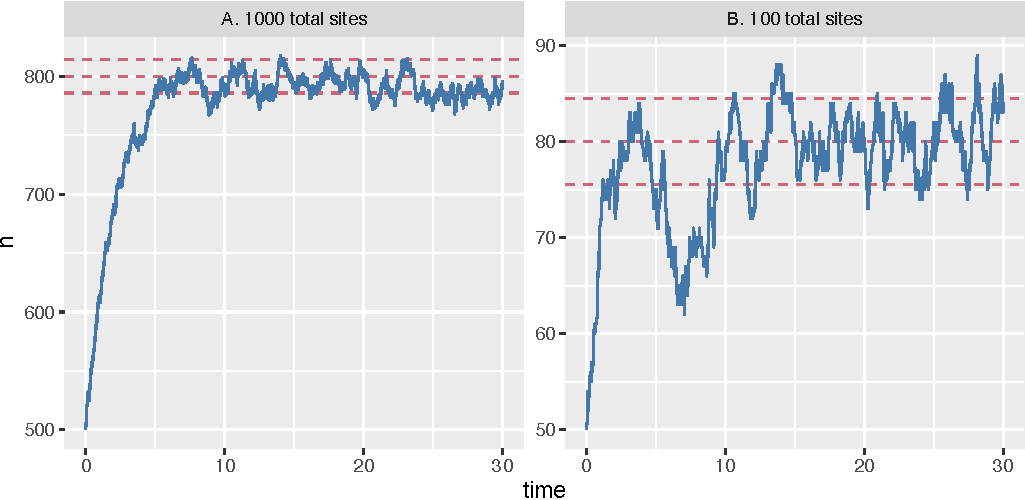
\includegraphics{paper_files/figure-latex/figure1-1.pdf}
\caption{Population dynamics from a Gillespie simulation of the Levins
model with large (N=1000, panel A) and small (N=100, panel B) number of
sites (blue) show relatively weaker effects of demographic noise in the
bigger system. Models are otherwise identical, with e = 0.2 and c = 1
(code in appendix A). Theoretical predictions for mean and plus/minus
one standard deviation shown in horizontal re dashed lines.}
\end{figure}

\hypertarget{conclusions}{%
\section{Conclusions}\label{conclusions}}

This review has explored three paradigms in how noise is viewed
throughout theecological literature, which I have dubbed respectively:
noise the \emph{nuisance}, noise the \emph{creator}, and noise the
\emph{informer}. Noise can be seen as a nuisance almost by definition:
in examining the origins of noise, we have seen how stochasticity is
introduced not because ecological processes are random in some
fundamental sense, but rather, because those processes are influenced by
a complex combination of forces we do not model explicitly. In this
view, noise captures all that additional variation that is separate from
the process of interest, and a rich array of statistical methods allow
us to separate the one from the other in observations and experiments.
By examining the origins of noise, we have seen that despite the complex
ways in this noise can enter a model, that a Gaussian white-noise
approximation (Kampen 2007; Black and McKane 2012) is often appropriate
given a limit of a large system size -- a fact often invokedn implicitly
but rarely derived explicitly from the theorems of Kurtz (1978) and
others.

In this context, noise does not act to create phenomena of interest
directly. The sudden transitions we seek to anticipate are still
explained by the deterministic part of the model -- bifurcations. But
nor is noise a nuisance that merely cloaks this deterministic skeleton
from plain view: rather, it becomes a novel source of information that
would be inaccessible from a purely deterministic approach. I believe
more examples of how noise can inform on underlying processes is
possible, but will require greater dialog between these world views.

\hypertarget{acknowledgements}{%
\section{Acknowledgements}\label{acknowledgements}}

The author acknowledges feedback and advice from the editor, Tim Coulson
and two anonymous reviewers. This work was supported in part by USDA
National Institute of Food and Agriculture, Hatch project
CA-B-INS-0162-H.

\hypertarget{references}{%
\section*{References}\label{references}}
\addcontentsline{toc}{section}{References}

\hypertarget{refs}{}
\leavevmode\hypertarget{ref-Abbott2011}{}%
Abbott, Karen C. 2011. ``A Dispersal-Induced Paradox: Synchrony and
Stability in Stochastic Metapopulations.'' \emph{Ecology Letters} 14
(11). Blackwell Publishing Ltd: 1158--69.
\url{https://doi.org/10.1111/j.1461-0248.2011.01670.x}.

\leavevmode\hypertarget{ref-Bartlett1960}{}%
Bartlett, Maurice S. 1960. \emph{Stochastic population models in ecology
and epidemiology}. London: Methuen; Wiley.

\leavevmode\hypertarget{ref-Bjornstad2001}{}%
Bjørnstad, O N, and Bryan T Grenfell. 2001. ``Noisy clockwork: time
series analysis of population fluctuations in animals.'' \emph{Science
(New York, N.Y.)} 293 (5530): 638--43.
\url{https://doi.org/10.1126/science.1062226}.

\leavevmode\hypertarget{ref-Black2012}{}%
Black, Andrew J, and Alan J McKane. 2012. ``Stochastic formulation of
ecological models and their applications.'' \emph{Trends in Ecology \&
Evolution}, March. Elsevier Ltd, 1--9.
\url{https://doi.org/10.1016/j.tree.2012.01.014}.

\leavevmode\hypertarget{ref-Boettiger2010}{}%
Boettiger, Carl, Jonathan Dushoff, and Joshua S. Weitz. 2010.
``Fluctuation domains in adaptive evolution.'' \emph{Theoretical
Population Biology} 77 (1): 6--13.
\url{https://doi.org/10.1016/j.tpb.2009.10.003}.

\leavevmode\hypertarget{ref-Coulson2001}{}%
Coulson, T. 2001. ``Age, Sex, Density, Winter Weather, and Population
Crashes in Soay Sheep.'' \emph{Science} 292 (5521): 1528--31.
\url{https://doi.org/10.1126/science.292.5521.1528}.

\leavevmode\hypertarget{ref-Coulson2004}{}%
Coulson, Tim, Pejman Rohani, and Mercedes Pascual. 2004. ``Skeletons,
noise and population growth: The end of an old debate?'' \emph{Trends in
Ecology and Evolution} 19 (7): 359--64.
\url{https://doi.org/10.1016/j.tree.2004.05.008}.

\leavevmode\hypertarget{ref-Gillespie1977}{}%
Gillespie, Daniel. 1977. ``Exact Stochastic Simulation of Coupled
Chemical Reactions.'' \emph{Journal of Physical Chemistry} 81.25:
2340--61.

\leavevmode\hypertarget{ref-vanKampen2007}{}%
Kampen, N.G. van. 2007. \emph{Stochastic Processes in Physics and
Chemistry}. Third. Amsterdam, New York, Oxford: North-Holland Publishing
Company.

\leavevmode\hypertarget{ref-Knape2011}{}%
Knape, Jonas, and Perry de Valpine. 2011. ``Are patterns of density
dependence in the Global Population Dynamics Database driven by
uncertainty about population abundance?'' \emph{Ecology Letters} 15 (1):
17--23. \url{https://doi.org/10.1111/j.1461-0248.2011.01702.x}.

\leavevmode\hypertarget{ref-Kurtz1978}{}%
Kurtz, Thomas G. 1978. ``Strong Approximation Theorems for Density
Dependent Markov Chains.'' \emph{Stochastic Processes and Their
Applications} 6 (3): 223--40.
\url{https://doi.org/10.1016/0304-4149(78)90020-0}.

\leavevmode\hypertarget{ref-Levins1966}{}%
Levins, Richard. 1966. ``The strategy of model building in population
biology.'' \emph{American Scientist} 54 (4): 421--31.

\leavevmode\hypertarget{ref-Levins1969}{}%
---------. 1969. ``Some demographic and genetic consequences of
environmental heterogeneity for biological control.'' \emph{Bulletin of
the Entomological Society of America} 15 (3). Entomological Society of
America: 237--40.

\end{document}


